\chapter{Introduction to lab equipment}\label{chap:intro}

The purpose of this lab is to introduce the computer programs and the
equipment you will be using in this course.  You will simulate the operation
of an open-loop motor scheme, illustrated in Figure~\ref{fig:openLoop1}\@.
\begin{figure}[htbp]
    \centering
    \begin{picture}(200,50)
        \put(0,22){\(u(t)\)}
        \put(20,25){\vector(1,0){30}}
        \put(55,5){\framebox(105,40)
            {\large\((\frac{d^2}{dt^2}+\frac{1}{\tau}\frac{d\theta}{dt})=k_Eu\)}}
        \put(165,25){\vector(1,0){30}}
        \put(196,22){\(\theta(t)\)}
    \end{picture}
    \caption{Open-loop motor schematic}\label{fig:openLoop1}
\end{figure}%
Hence, the differential equation governing the system is:
\begin{equation}\label{eq:motor}
    \frac{d^{2}\theta}{dt^{2}}+\frac{1}{\tau}\frac{d\theta}{dt}=k_E u.
\end{equation}
We are interested in the angle, \(\theta \), and the angular velocity,
\(\omega=\frac{d\theta}{dt}\), of the motor shaft.  By the end of the lab,
you will have enough data to calculate the motor time constant, \(\tau \), and
torque constant, \(k_{E}\).

\section{Key Concepts}
As the first lab is primarily used to have students familiarize themselves with
laboratory equipment, it does not focus heavily on course related material.
However, this lab will introduce you to certain applications of Matlab and Simulink
which will be used continuously throughout all 9 labs in this manual. Simulink is a
program that allows us to simulate a system, define an input to this system,
and send the systems output to Matlab. In these labs our system will be a DC motor,
to which we will be applying various inputs and observing the outputs. Simulink will
also be used continuously throughout the project portion of the course.

You will be using Matlab throughout this course, so start using some best practices. Some useful tips:
\begin{enumerate}
    \item \emph{Always} start a script. Whether you are trying to generate plots, simulate dynamics, or do calculations, it is significantly easier to edit, re-use, re-run code in a script as opposed to the workspace.
    \item Save your Simulink models to the cloud. This will save you from having the rebuild your model each week.
    \item Use a semicolon ``;'' to surpress outputs.
    \item You can create Section in your script using double percent signs.
    \item The \verb|plot| function can handle multiple \(x,y\)-tuples. Use this to your advantage. The only requirement is that each vector pair has to be the same \emph{length}. You can have multiple \(y\) values for one \(x\) vector.
\end{enumerate}
\section{Prelab}

It is assumed that the students of this course will have working knowledge of
personal computers. Before you go into the lab, you should read the
following:
\begin{itemize}
    \item Appendix~\ref{chap:MATLAB}: \textsf{Matlab};
    \item Appendix~\ref{chap:hardware}: Lab equipment;
    \item Appendix~\ref{chap:simulink}: \textsf{Simulink};
    \item Section 1.2 from the course text.
\end{itemize}

Before the lab, you must solve the ODE given in Equation~\ref{eq:motor}, for a constant input \(u(t)=1\), using an appropriate technique.
Remember that for an equation of the form \(\frac{dy}{dt} + P(t)y(t) = Q(t)\), the integrating factor \(\mu(t) = e^{\int P(t)dx}\). Or, you can use Laplace Transformations.

You will be expected to be able to look up material in the appendices during
the course of the various labs, so it is best that you be familiar with what
is in them.  If you are already familiar with any of the topics, you may skip
that section.

\section{Procedure}

The following steps should be followed to set up the simulink models to
properly communicate with the hardware.  You should perform the following
steps \emph{before} adding any blocks to your simulink model to avoid
manually configuring each block in your model.  Concerning any check boxes,
if it is not explicitly stated that you should check a box then it
\emph{must} be left unchecked.
\begin{enumerate}
    \item Create the directory
          \begin{center}
              \verb|C:\Documents and Settings\<Qlink ID>\My Documents\MATLAB|
          \end{center}
          if it does not already exist.
    \item Start \textsf{Matlab}.
    \item Type \verb|simulink| at the prompt.
    \item Click \verb|File|\(\to \)\verb|New|\(\to \)\verb|Model| to create a new empty
          simulink model.
    \item Build a \textsf{Simulink} model (the following steps will guide you
          through this) as shown in Figure~\ref{fig:lab1}\@.
          \begin{figure}[htbp]
              \centering
              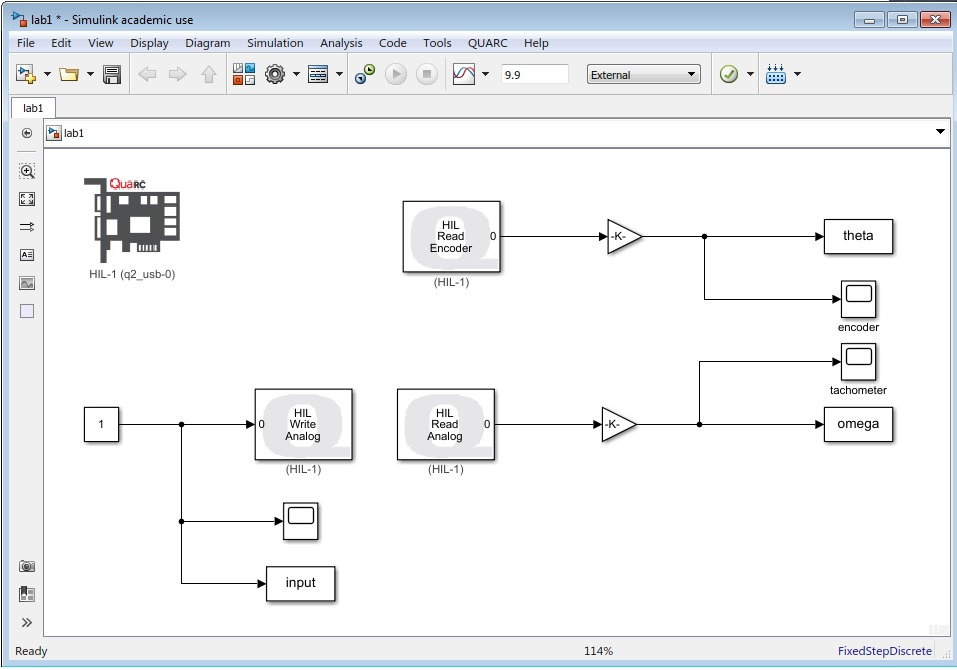
\includegraphics[width=0.9\textwidth]{pix/lab1.PNG}
              \caption{\textsf{Simulink} model for Lab~\ref{chap:intro}}\label{fig:lab1}
          \end{figure}%
          The model applies a constant voltage to the servomotor.  The encoder is
          employed to acquire the angular position (\(\theta \)) and the tachometer is
          used to acquire the angular velocity (\(\omega \)) as functions of time.
    \item Make a new folder on the hard drive under the name or number of your
          group and save your model under the name \verb|lab1_name_of_your_group.mdl|.
          Save all files created (e.g., model file, plots) in each lab session in that
          folder.  It might be a good idea to create a folder for each lab session as
          well.

    \item Drag the \verb|HIL Initialize| block from the library window into the
          model.  You can find this block under:
          \begin{center}
              \verb|QuaRC Targets|\(\to \)\verb|Data Acquisition|\(\to \)\verb|Generic|\(\to \)\verb|Configuration|
          \end{center}
    \item Double click on the new \verb|HIL Initialize| block in your model to
          configure the parameters.
          \begin{enumerate}
              \item Main Tab
                    \begin{itemize}
                        \item Board Type = \verb|q2_usb|
                    \end{itemize}
              \item Encoder Inputs Tab
                    \begin{itemize}
                        \item Encoder Input Channel = \verb|[0]|
                        \item Encoder Quadrature = \verb|[4]|
                        \item Encoder Frequency in Hertz = \verb|[ ]|
                        \item Initial Encoder Counts = \verb|0|
                        \item Check box \verb|Set encoder input parameters at model start|
                        \item Check box \verb|Set initial encoder counts at model start|
                    \end{itemize}
              \item Analog Outputs Tab
                    \begin{itemize}
                        \item Analog Output Channels = \verb|[0]|
                        \item Initial Analog Outputs = \verb|0|
                        \item Final Analog Outputs = \verb|0|
                        \item Analog Outputs on Watchdog Expiry = \verb|0|
                        \item Check box\\
                              \verb|Set initial analog outputs when switching to this model|
                        \item Check box \verb|Set final analog outputs at model termination|
                        \item Check box\\
                              \verb|Set final analog outputs when switching from this model|
                    \end{itemize}
          \end{enumerate}

    \item Click \verb|Apply| and then \verb|OK| to close the properties dialog box.

    \item Once the \verb|HIL Initialize| block is set up properly, you can add
          blocks to your simulink model to read and write analog signals to the
          interface board.  The main blocks of interest are \verb|HIL Read Encoder|,
          \verb|HIL Read Analog| and \verb|HIL Write Analog|, which replace the old
          blocks \verb|Encoder Input|, \verb|Analog Input| and \verb|Analog Output|,
          respectively.  Consult the instructions to see which blocks to use in each
          lab. There are no \verb|calibration|, \verb|encoder|, or \verb|tachometer|
          blocks.  These blocks are simply ``gain'' or ``scope'' blocks which have been
          renamed.  It is always best to refer to the block pictures instead of the
          block names.  These blocks can be found at
          \begin{center}
              \verb|QuaRC Targets|\(\to \)\verb|Data Acquisition|\(\to \)\verb|Generic|\(\to \)\verb|Immediate I/0|
          \end{center}
          \begin{center}
              \verb|Simulink|\(\to \)\verb|Commonly used blocks|
          \end{center}
          When using the HIL \verb|Read Analog| block, make sure that the correct
          channel is set (channel \verb|0|).
          \begin{figure}[htbp]
              \centering
              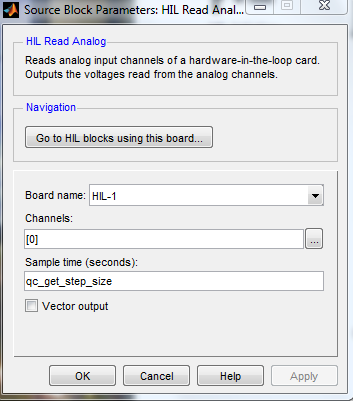
\includegraphics[width=0.5\textwidth]{pix/hil-read-analog-block.PNG}
              \caption{HIL \texttt{Read Analog} block settings}\label{fig:hilrab}
          \end{figure}
          \begin{figure}[htbp]
              \centering
              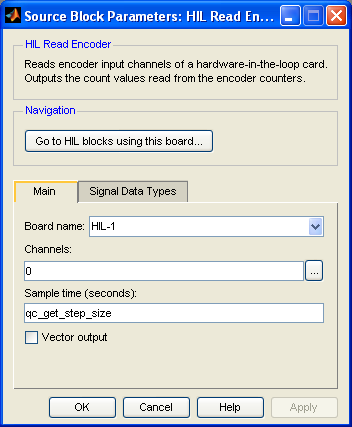
\includegraphics[width=0.5\textwidth]{pix/hil-read-encoder-block.PNG}
              \caption{HIL \texttt{Read Encoder} block settings}\label{fig:hilreb}
          \end{figure}
          \begin{figure}
              \centering
              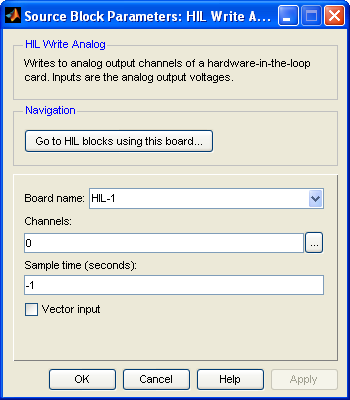
\includegraphics[width=0.5\textwidth]{pix/hil-write-analog-block.PNG}
              \caption{HIL \texttt{Write Analog} block settings}\label{fig:hilwab}
          \end{figure}
    \item The input and output channel numbers in the \textsf{Simulink} blocks should
          match the channels used on the terminal board. Refer to
          Figures~\ref{fig:hilrab}\@,~\ref{fig:hilreb}\@, and~\ref{fig:hilwab} for the
          correct channels.
    \item \label{enum:parameters} The calibration factors need to be set so that %chktex 24
          servomotor angular position and velocity are acquired in appropriate units. Double
          click on the \verb|Gain| block for the encoder and set the gain to \(-\frac{2\pi}{4096}\).
          Similarly, set the Tachometer gain to \(\frac{100\pi}{63}\). These values can be found in
          Table~\ref{tab:conversionFactors} in Appendix~\ref{chap:hardware}.
    \item The \verb|To Workspace| block can be found at
          \verb|Simulink|\(\to \)\verb|Sinks|.  Drag this block into your workspace and
          connect it to the variable you wish to save.  Double click on the block to
          configure it.  Choose a good variable name and, in the \verb|save format|
          drop down menu, select \verb|Structure with time|.
    \item Click on \verb|Simulation|\(\to \)\verb|Configuration Parameters| from
          your \textsf{Simulink} screen (or \verb|Ctrl+E|).  Make sure you are using
          \verb|fixed-step| integration and choose \verb|ode 4| as your method.
    \item Select \verb|Set default options| from the \verb|QuaRC| drop down menu.
    \item Select the \verb|External| mode option from the drop down menu in the toolbar.
          Note that \verb|External| mode is only necessary for labs that use the Servomotor.
    \item In the toolbar, change ``in'' to 5 and press enter. This is the simulation time. A note: the software seems to forget all data older than 10 seconds during the simulations, so for the purpose of this lab, we set the \verb|Stop Time| to 5 seconds.
    \item Double click on the \verb|Encoder| and \verb|Tachometer| blocks to open
          the plots.  More details on viewing real-time results can be found in
          Appendix~\ref{chap:simulink}\@.
    \item Select \verb|Builld from the \verb|QuaRC| drop down menu.  Wait for
          building to be completed before preceding to next step. Progress can be seen
          in the Command Window. The keyboard shortcut for building is \verb|Control+B|
    \item Provided there are no compilation errors, select
          \verb|Connect to Target| from the \verb|Simulation| menu.
    \item Select \verb|Run| from the \verb|Simulation| menu, or click
          the black play button in the toolbar. The keyboard shortcut for this is \verb|Control+T|.
    \item Data will automatically be saved from the \verb|To Workspace| blocks.
    \item Plot it with the command
          \begin{center}
              \verb|plot(varname.time,varname.signals.values)|
          \end{center}
          replacing ``\verb|varname|'' with the variable name you chose when
          configuring the \verb|To Workspace| block.  Use the \verb|plot| command in
          \textsf{Matlab} to plot data from the \verb|Encoder| and the
          \verb|Tachometer|.  Details on plotting in \textsf{Matlab} are discussed in
          Appendix~\ref{chap:MATLAB}.  Remember to give the plots appropriate title
          and axis labels and print these plots. What is the steady state angular
          velocity?  Are the results from these plots as you expected?
    \item Now that you have obtained the steady-state value from the angular
          velocity plot, you are ready to determine the actual value of the motor time
          constant, \(\tau \), and the torque constant, \(k_{E}\).  Recall that solving
          the differential equation~(\ref{eq:motor}) with zero initial condition yields
          \begin{align}\notag
              \omega(t)= & \;\dot\theta(t),             \\\label{eq:motorSoln}
              \omega(t)= & \;k_{E}\tau (1-e^{-t/\tau}),
          \end{align}
          and so the steady state value is just \(k_{E}\tau \).
    \item First, determine the steady state value and the constant \(\tau \) from
          the angular velocity plot.  You can find \(\tau \) by using the steady state
          value and finding the value of \(\omega(t)\) when \(t=\tau \).
    \item Next, determine \(k_{E}\) using Equation~(\ref{eq:motorSoln}) and the
          constants obtained in the last step.  You might need to zoom in to the
          appropriate portion of the graph to see the result clearly.
    \item Once you have confirmed with the TA that you have obtained the correct
          value of the constants, print a copy of the plot that you zoomed in on.
    \item Save all files in the folder you created.  Hand in all the plots you
          printed during this lab session and along with it the work to show how you
          have obtained the two constants.  Please make sure the names and student
          numbers of all your group members are on the first page.
\end{enumerate}
The constants obtained in this lab will come in handy in the future, so make
sure you check with the TA that you have obtained the correct (or reasonably
close) value before you leave.

\textbf{Save your Simulink model to an accessible location. You will need it next week.}

\section{Deliverables}

Prepare a brief write up describing what you learned from this lab.
This does not need to be a formal report, but all material should be presented in
a clear and logical manner, with concise descriptions where necessary. Include
the following/answer the following questions:
\begin{enumerate}
    \item Plots of motor position (\(\theta \)) and velocity (\(\omega \)) with respect to time. Make sure you label your axes appropriately.
    \item What is the steady state angular velocity (in rads/s) of the motor?
          Does this correlate to the value obtained using the encoder plot?
    \item Determine the motor constant \(\tau \). Include a plot at t = \(\tau \) (use proper units).
    \item Determine the motor torque constant, \(k_E\) (include units). Show your calculations.
\end{enumerate}

%%% Local Variables: 
%%% mode: latex
%%% TeX-master: "lab-manual"
%%% End: 
